\chapter{Introduction}
\label{INTRODUCTION}

Wireless networks utilize radio waves instead of wires to carry information, which makes seamless coverage and mobility possible to realize.
%Wireless networks use have experienced unprecedented growth in the past few decades and will going on evolving in the future.
After decades of fast growth, there have been many wireless standards designed for different purposes.
For example, wireless personal-area network (\gls{wpan}) connects devices which locate within a short range of 10 meters.
The WPAN specifications \ie Zigbee, Bluetooth are specified by IEEE 802.15 standards.
Wireless local-area network (\gls{wlan}) enables mobile user to connect to to a local area network (LAN) through wireless connection within a range of one hundred meters, where the technologies are specified by the IEEE 802.11 group of standards.
WiFi is a successful realization of WLAN technology, which is based on IEEE 802.11 standard.
Wireless metropolitan-area network (\gls{wman}) provides connection with broadband speeds and larger coverage (from one hundred meters to several kilometres), where the technologies adopted are specified by IEEE 802.16.
Third generation (\gls{3g}) mobile communication systems have seen widespread deployment around the globe, which provide people with higher data rates and better quality of service (\gls{QoS}) for different services.
These technologies and standards, along with many others~\cite{Molisch:2011:WC:1984860}, fit different needs of various applications.


Due to the propagation characteristics and regulations, the electromagnetic spectrum which spans from 8.3 kHz to 3000 GHz is suitable for commercial application.
These spectrum is divided into bands (also referred as channels) and allocated to different networks and services.
For example, WiFi and Bluetooth devices communicate in the 2.4 GHz radio frequency (\gls{rf}) industrial, scientific, and medical (\gls{ISM}).
Wimax networks work from 2 GHz to 66 GHZ in the RF spectrum.
%In the following, we introduce how is the spectrum accessed by different services.
%
As one kind of limited and precious resource, radio spectrum is strictly regulated by the national administration.
The channels are assigned or leased by governments to different operators and entities.
In most cases, the operators pay high price for the commercial usage of certain spectrum, and the usage is exclusive for them~\cite{Spectrum_Management07}.
This spectrum management policy rules out the unlicensed users to use the spectrum, thus strictly protects the interest of the spectrum licensees.
This spectrum access module is referred as \textit{exclusive use model}~\cite{zhao_survey_DSA_2007}, and is the mainstream of spectrum access worldwide, and many existing wireless applications work on the licensed spectrum.
For instance, the second-generation (2G) wireless cellular network \gls{gsm} (global system for mobile communications) in Europe works with GSM-900 band (from 890 MHz to 960 MHz) and GSM-1800 (1710 MHz to 1880 MHz), and the third-generation (3G) wireless cellular network works from 1.8 GHz to 2.4 GHz~\cite{wireless_communicatioins2001}.
The excludability of licensed spectrum can also be open to other user with conditions.
The spectrum licences either sell and trade the licensed spectrum, or dynamically use the spectrum within a certain region according to different traffic patterns~\cite{dsa_traffic_2000}.

Open spectrum access~\cite{osa_Noam_1995} is proposed in 1995 for full openness of entry, which allows access to spectrum through access fees which are determined by demand and supply.
It is claimed that open spectrum access yields benefits, as for spectrum licensees, the fixed costs on securing the licensed spectrum can be converted into marginal costs, and for the market, the incentives for collusive pricing can be eliminated.
But as the \textit{openness} here is fully controlled by the licensees, this spectrum usage is still exclusive .

%
In contrary to exclusive use model, certain spectrum are assigned for open sharing for peer users, the representative example is the unlicensed ISM radio band, which supports versatile wireless applications and a prosperous industry, \ie Wi-Fi.
Many spectrum sharing strategies are proposed to cope with the technical challenges~\cite{Ko_DistributedCA}.

%
The proliferation of wireless network constantly arises urgent demand on bandwidth and throughput since the first generation of telecommunication in 1980s, which accordingly encourages the efficient use and reuse of the electromagnetic spectrum.
The next generation of telecommunication technology \gls{5G}, which is reported to come true in 2020, requires a leap forward of spectrum efficiency~\cite{5G_2014}.
The resorted applications under the label of 5G~\cite{5directions5G_2014}, \ie machine to machine communication, internet of things, etc, requires high speed and lower investment cost, but this is changeling as the achieved capacity approaches Shannon capacity, and most spectrum are licensed.
Meanwhile, the actual spectrum usage measurement conducted by FCC tells that at many locations or time, the licensed spectrum is idle~\cite{FCC_spectrumEfficiency_2002}, and there exists a large number of spectrum bands which have considerable dormant time intervals ~\cite{Akyildiz06survey}.

%
To seek more opportunities from spectrum, it is natural to consider opening the licensed spectrum to unlicensed users to use, when the spectrum is not been used by licensed users, or the the licensed users' operation is not hampered.
%\section{Hierarchical Spectrum Access}
%\label{hierarchical}
We adopt the terms proposed in~\cite{zhao_survey_DSA_2007}, and call this spectrum usage policy as \textit{hierarchical access model}, where licensed users are called primary users (\glspl{PU}), and unlicensed users are named as secondary users (\glspl{SU}).
Hierarchical access model gives a promising solution to the reclamation of new electromagnetic spectrum and the improvement of spectrum efficiency.




%\subsection{Spectrum Access Etiquette in Cognitive Radio Network}
%
%%CR users utilize the unused licensed spectrum opportunistically and meanwhile avoid interfering licensed users.
%%This new spectrum usage paradigm imposes great challenge to the CR users, including how to detect the licensed users and afterwards decide on the suitable spectrum and on which interact with other CR users.
%
%%Before the emerging of cognitive radio technology, spectrum is allocated in a fixed way, \ie certain chunk of spectrum is exclusively licensed to an certain entity by administration body.
%%The equipments which are given the license to utilize the spectrum is called licensed users, while the others which called unlicensed users are not allowed to work on the that part of spectrum.
%%This paradigm rigidly protects the benefit of licensed users, but it results in underutilization of spectrum.
%%Due to the drastic increase of mobile data applications there is an urgent demand on spectrum resources. 
%%Traditionally, frequency bands have been assigned exclusively to licensed bodies which can occupy the spectrum whenever there is information to be transmitted. 
%
%%This static spectrum utilization has been proven to be suitable for many systems and applications. 
%%However, as mobile networks have proliferated drastically over the last thirty years, this exclusive assignment has created a significant shortage of spectrum today. 
%
%Licensed users access their allocated spectrum band whenever there is information to be transmitted, in contrary, CR users are only allowed to access licensed spectrum after validating the channel is idle or the primary user is not to be affected if they operate on the licensed spectrum.
%In this thesis, licensed users are referred as primary users, and CR users are denoted as secondary users.
%
%The assessment of spectrum is a bone of contention for primary/secondary users and administration bodies.
%Spectrum sensing on secondary users is one common method to validate spectrum availability especially in research domain~\cite{crnsensing_09}.
%%Secondary users should monitor the spectrum of interest actively and autonomously to detect primary users' appearance.
%%Primary users can be detected by judging the primary users' signal power, spectral correlation or beacons.
%%Spectrum sensing requires sophisticated technologies when primary users' signal is weak.
%%Primary detection can be improved by learning technologies or cooperation among multiple secondary users~\cite{coorperativeSensing_Akyildiz11}.
%Another way to protect the primary users from being affected by secondary users' operation relies on location identification and certain operating rule set.
%Based on the global information of primary users' location and terrain information, centralized controller regulates that the secondary users at certain locations are restricted to operate on a few certain spectrum bands and with limited transmit power~\cite{whitefi09}.



%In contrast, CR users (forming cognitive radio networks, abbreviated as CRN) 
%This refers to the process of sensing a particular channel and verifying (with a previously specified probability of error) that it is not used by a primary user currently  [cite spectrum sensing].
%This form of spectrum sharing is also referred to as opportunistic spectrum access~\cite{Akyildiz06survey}.

%Such co-existence with primary users imposes great challenges for the CR users.
%On the first hand, CR users should be able to sense the channel to avoid interfering primary users.
%it is fairly easy to see that the sensing ability of secondary users plays an important role in the harmonious co-existence of primary and secondary users~\cite{09spectrumSensing_survey}.





\section{Cognitive Radio Network}
%\cite{spectrumSharingGames_interference_stackelberg_2009, spectrum_sharing_games_2010} spacial opportunistic allocation.

A cognitive radio network is composed with secondary users and work with the hierarchical access model.
Throughout this thesis, we use \textit{cognitive radio networks} to compound the networks composed with secondary users, 
% which work in either spectrum underlay or spectrum overlay style.
there are two reasons, firstly, this name explicitly tells a distinctive property of the devices in the networks, which is their cognition ability to their environment, secondly, cognitive radio has become a synonym of the technology employed in the hierarchical spectrum access paradigm in academia and industry in the recent years.

%The dilemma that spectrum scarcity coexists with spectrum underutilization promotes cognitive radio (CR) as a promising technology to make full use of spectrum and accordingly solve the spectrum shortage problem.

The definition of cognitive radio evolves with the development of radio technology and regulations.
We choose two representative definitions to draw a full picture of cognitive radio.
Cognitive radio (\gls{CR}) is firstly proposed by Mitola III who defines the concept of CR in his dissertation~\cite{2000mitola_cognitive_radio} as follows:
%
\blockquote{The point in which personal digital assistants (\glspl{PDA}) and the related networks are sufficiently computationally intelligent about radio resources and related computer-to-computer communications to detect user communications needs as a function of use context, and to provide radio resources and wireless services most appropriate to those needs.
}

FCC (Federal Communications Commission in U.S.) describes CR~\cite{FCC_03-322} as,
\blockquote{
a radio that can change its transmitter parameters based on interaction with the environment in which it operates. $\ldots$
This interaction may involve active negotiations with other spectrum users and/or passive sensing and decision making (smart radio) within the radio. 
The majority of CRs will probably be SDRs~\footnote{software defined radio is a radio communication system which is able to receive any modulation across a large frequency spectrum, and transmit on desired spectrum band.}, but a CR does not necessarily use software, nor does it need to be field programmable.
}

The first definition depicts the functionalities of cognitive radio devices, and the second one mentions the relationships between cognitive radio users and the network which it resides.
In this dissertation, we see cognitive radio as a device which is able to sense, detect, learn and monitor the surrounding radio frequency environment, or to access a certain database to retrieve primary users' information, so as to reconfigure its radio operating parameters (\eg center frequency, bandwidth and transmit power) on the fly to avoid interfering primary users.
Cognitive radio may only practice one portion of the aforementioned functionalities according to actual situation.
%Apparently, the cognitive radio users which conduct spectrum sensing are usually work with spectrum overlay paradigm (introduced in Section~\ref{overlay}), and the cognitive radio users which have means to get information of primary users are suitable to work with spectrum underlay paradigm (introduced in Section~\ref{underlay}).
%Based on this definition, throughout this thesis the secondary users working with both spectrum underlay and overlay are named as cognitive radio users, besides, the cognitive radio network is deemed to be composed with cognitive radio users, whose acronym is \gls{CRN}.
Based on this definition, the cognitive radio network is deemed to be composed with cognitive radio users, whose acronym is \gls{CRN}.

Throughout this dissertation, we use several different terms to denote cognitive radio devices, \ie, cognitive radio users, secondary users, or secondary nodes in different contexts.
In particular, when we want to stress the devices' cognitive ability on their environment, we use the term cognitive user or CR user, when we discuss spectrum sharing, and want to indicate the passiveness of the devices in terms of spectrum, we call them secondary users. 
If the CRN is depicted as a graph, and we emphasis on the network topology, then the term node will be used.


\subsection{Functionalities of Cognitive Radio}
To adapt to the dynamic spectrum environment and make use of the available licensed spectrum, cognitive radio users %need to manage the available spectrum by conducting a series of functionalities sequentially, \ie detecting the available spectrum with spectrum sensing, selecting the proper spectrum for communication, communicate with other secondary users using certain spectrum band, and moving to another channel when the current working channel is not usable due to primary user's appearance.
These functions are incorporated into so called cognitive cycle as described in~\cite{Akyildiz09}.

\subsubsection{Spectrum Sensing}
To know which chunk of spectrum is available is the foundation of spectrum management.
In underlay spectrum usage scenario, CR users get to know the available spectrum by means of spectrum sensing.
In overlay spectrum usage scenario, secondary users can in principle access all the licensed spectrum.
In this procedure, quality of the available channels is determined with several parameters, \ie bandwidth, operating frequency, path loss, wireless link errors, link layer delay, and the upper bound of interference on the primary user working on that channel, which decides the maximal permissible transmission power of secondary users.
Besides, the statistical behaviours of primary users is also an important factor.

Spectrum administration bodies FCC of U.S.~\cite{FCC_2010_sedond_memorandumm} and Electronic Communications Committee (\gls{ECC}) in Europe~\cite{ecc159} encourage to adopt both spectrum sensing and location based method.

\subsubsection{Spectrum Decision}
After knowing the available spectrum, CR users select the most appropriate band according to their requirements on quality of service (QoS).
This procedure involves considering the statistical behaviours of the primary users so as to accessing the channel quality fairly.
The available licensed spectrum which spans a wide frequency band exhibits different characteristics~\cite{spectrum_decision_TMC11}.
Based on the requirements of interested communication, CR users need to identify the characteristics of the spectrum, which include channel quality (channel capacity, error rate, path loss, etc.)~\cite{spectrum_decision_TMC11}, channel switching delay~\cite{channel_switch_delay11}, and channel holding time, \ie the expected time duration that the primary users don't occupy the channel before any one occupies again.

Some works in research community model the spectrum availability with stochastic or statistical model, which is helpful when deciding which channel to use.
\cite{Discrete-Time_Spectrum_Occupancy_Model_DySPAN_2011} proposes discrete Markov chain and adjusts duty cycle models to describe the availability of licensed spectrum for GSM on 900/1800 MHz.
\cite{Wellens200910} models the channel holding time with geometric and log-normal distributions.
Statistics of previous sensing results is used to predict spectrum state in the future~\cite{spectrum-discovery-tmc08}.
Such models provide more complete information on the availability of the licensed channels.




\subsubsection{Spectrum Sharing}
Then secondary users are to make use of these channels selected in the spectrum decision procedure, and share the spectrum with both the primary users and the other secondary users.
As there may be multiple secondary users trying to use the same channel, spectrum sharing is important to coordinate the behaviour of secondary users to avoid deteriorating the performance of secondary users.
Spectrum sharing involves choosing proper channels to mitigate co-channel and adjacent interference~\cite{ca_crn_survey_2013}, or adjusting transmission power to reach compromise between transmitter's and other secondary users' performance~\cite{pa_crn_survey_2012}, or adopting a certain media access paradigm to use the spectrum fairly and efficiently.
Spectrum sharing also involves the concerns from primary users, \ie when many secondary users work on the same channel, the accumulated interference caused by secondary users could exceed the interference threshold on primary users.
%\todo[inline]{spectrum opportunity, detection, tracking, exploitation (whether to access, how to access, sharing),  tazhaosurveyDSA2007.}

%According to \cite{08crn_survey}, 	
%After assessing RF environment or geographic location, secondary users adjust their operational parameters such as frequency, modulation schemes and transmit power, in order to support QoS aware communications, this process is referred as spectrum decision and spectrum sharing~\cite{08crn_survey}.
%In this thesis, spectrum decision and sharing consist the major issue discussed in this thesis.

\subsubsection{Spectrum Mobility}
When one primary user starts to work on a certain channel from idle state, a secondary communicating pair working on the this channel should change their operating channel to another one, where no primary user is detected working on the new channel.
This hand off process between channels is called spectrum mobility, which is critical to maintain the communication and network topology for CRN.  





\subsection{Spectrum Sharing in CRN}
\label{spectrum_sharing}
Spectrum sharing can be divided into two categories, the spectrum sharing between the primary users and secondary users, and the one among the secondary users.
The first category is fundamental to the hierarchical access model, as it poses threat of interfering primary users.
The second category decides the services that people can obtain from CRN.
Thus, spectrum sharing largely defines the challenges and considerations one cognitive radio network faces.


\subsubsection{Spectrum Sharing between Primary and Secondary Users}
As to the spectrum sharing between primary users and secondary users, there are two models, spectrum underlay and overlay.
The two models origin from the distinctive understandings of people as to the hierarchical access model, and the different claims on how to effectively protect the primary users' interests.
%\subsection{Spectrum Underlay and Spectrum Overlay}
%Spectrum sharing can be classified by network architecture and spectrum allocation behaviour~\cite{Akyildiz09} respectively.


\begin{itemize}
\item \label{underlay}  Spectrum underlay:
Working with \textit{spectrum underlay}, secondary users are allowed to transmitting even when primary users are detected (or known via other means) to be operating on the same chuck of spectrum, as long as the interference generated by secondary users on the primary receivers is under a threshold.
Spectrum underlay restricts the secondary users' transmission power, but secondary users are still able to achieve high data rate in short range.
When implementing spectrum underlay, secondary users are allowed to operate in the close vicinity of primary users when the interference caused on primary users is carefully watched~\cite{Ellingsaeter2012_Increasing_Available}.
For instance, a there is a device need to monitor the interference level caused on primary users, and the secondary user need to be aware of this information via certain means~\cite{HoangPowerChannel2010}.

Spectrum underlay is usually conducted in a centralized controller, which has global knowledge of primary users' locations, the attenuation between all secondary transmitters and all primary receivers.
Then the centralized controller obtains the maximum permitted transmission power by solving an optimization problem where the interference generated by secondary users doesn't exceed the thread of primary users serves as one constraint.
%secondary users at certain locations are restricted to operate on a few certain spectrum bands and with limited transmit power~\cite{whitefi09}.
%Given the attenuation between all secondary transmitters and all primary receivers and their locations, when the interference threshold is known, the maximal permitted transmission power levels of secondary transmitters can be obtained with linear programming.
Working with spectrum underlay paradigm, spectrum sensing functionality on secondary users becomes auxiliary~\cite{FCC_2010_sedond_memorandumm, ecc159}.





\item \label{overlay} Spectrum overlay:
The other approach is \textit{spectrum overlay}, where secondary transmitters are only allowed to transmit when the primary users are detected as being idle, and the spectrum should be vacated if a primary user is detected transmitting.
This paradigm requires secondary users to sense the spectrum of interest pre-actively to detect primary users' appearance, accordingly entails burden on secondary users especially on the aspect of spectrum sensing.
The spectrum sensing metrics include received primary users' signal power, spectral correlation or beacons~\cite{crnsensing_09}.
Spectrum sensing requires sophisticated technologies when primary users' signal is weak, and can be improved by learning technologies or cooperation among multiple secondary users~\cite{coorperativeSensing_Akyildiz11}.
When spectrum sensing accuracy can be guaranteed above certain threshold, transmission power restrictions can be removed from  secondary users.
\end{itemize}

In summary, spectrum overlay can be seen as time division among primary and secondary users, as comparison, spectrum underlay can be seen to be space (or power) division.
Figure~\ref{underlay} shows a spectrum sharing scenario where the primary users are the TV systems.
Secondary user 1 works in spectrum overlay by detecting and then using the spectrum, secondary user 2 works in spectrum underlay by refraining its transmission power.
	\begin{figure}[h!]
	  \centering
	  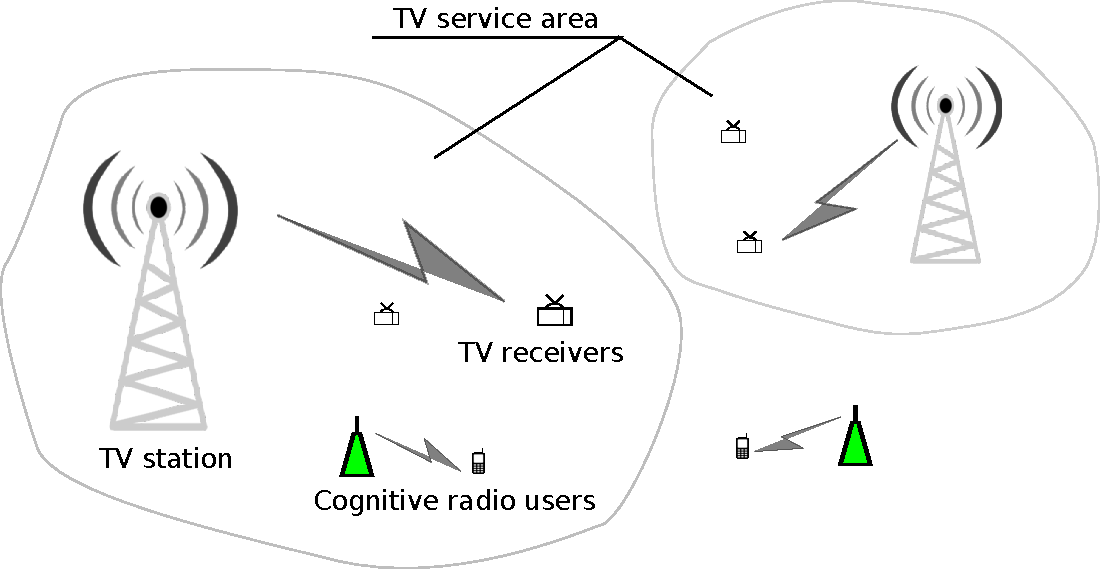
\includegraphics[width=0.75\linewidth]{underlay.pdf}
	  \caption{An illustration of underlay and overlay spectrum usage. The hull shows the range of a TV service area.}
	\label{underlay}
	\end{figure}

\subsubsection{Spectrum Sharing among the Secondary Users}
Among the secondary users, there is also competition on transmission power, spectrum bands or transmission time slots.
When we put the consideration on protection of primary users aside, spectrum sharing among the second users is similar with the counterpart problems in the conventional wireless networks, \ie ad hoc networks, cellular networks, etc..
In CRN, spectrum sharing among the secondary users can be conducted with either cooperative or non-cooperative manner.
As to cooperative spectrum sharing, secondary users take into consideration of the caused interference on other secondary users when deciding their spectrum usage.
This pattern usually requires cluster structure to facilitate the negotiation of users in a neighbourhood~\cite{Chen07}.
Whereas with non-cooperative spectrum sharing, secondary users only consider the performance of their own.



%Secondary users' operation is restricted on certain spectrum bands and transmit power should be below certain threshold according  to their locations, and spectrum sensing ability is also required.





%\subsection{Operation Models of Spectrum Sharing in CRN}
%\label{operation_model}
From the perspective of network operation, spectrum sharing can be classified as centralized and distributed spectrum sharing.

%Centralized spectrum decision doesn't work well outside the TV channel scenario.




\section{Solutions in CRN and Game Theory}
\label{gametheory_crn}

We introduce the problems and corresponding solutions in CRN, and the application of game theory int he problem solving.

\subsection{The solutions in CRN}
We introduced the solutions in CRN, which are categorised as centralized and distributed.

\subsubsection{Centralized Scheme}
Centralized spectrum sharing is conducted on a centralized entity to decide the secondary users' strategies to operate in the CRN.
There is a considerable number of centralized approaches proposed for spectrum sharing in cognitive radio network, and the global optimality is reported as to different objectives in certain cases.
%
The centralized solution is usually realized by formulating the communication problems into optimization problems.
Let us take the resource allocation problem in CRN as example.
The resource refers transmission power, spectrum, transmission time, etc..
The objective can be the following, improving the overall SINR of secondary users, mitigation of co-channel interference caused secondary users, minimization of transmission power, etc,.
The constraints can be one or several of the following, the interference caused by secondary users on primary users is below a threshold, the transmission power is restricted by the maximum transmission power, or the number of spectrum bands allowed for secondary users to use.
There is a good number of research in this regard~\cite{resource_allocation_crn_Ahmad_2015}~\cite[Chapter~6]{Han:2008:RAW:1457343}.
%There has been a good number of works in this regards~\cite[Chapter~6]{Han:2008:RAW:1457343}.

When the formulated problems are linear programming, or convex programming problems, the optimal is easy to obtain.
When convexity doesn't held, there all some skills to convert the problem into convex ones, \eg a $\log$ change of variables turns an apparently non-convex problem into a convex one.
When integer variables are involved in the optimization, \eg in problem of channel assignment, or scheduling, the optimization problem is very difficult to solve.
In this occasion, swarm intelligence algorithms can be applied to obtain sub optimal result, \ie simulated annealing~\cite{simulated_annealing_09, Tang20122690}, generic algorithm~\cite{Chen_2010} and ant algorithm~\cite{he_2012}.

Centralized scheme is suitable in certain scenarios, \eg when the primary users are TV stations and receivers which work on certain channels for hours of time, spectrum can be seen as constant. 
When the secondary users access the spectrum in underlay paradigm, they need to take care not to cause more interference than threshold on primary users.
In this case the channel usage, \ie working channel and transmission power, can be decided on the centralized controller.
%
Nevertheless, centralized solution is not suitable in many scenarios of CRN.
First, central authority or controller is not available in many CRNs, \eg cognitive radio ad hoc network (\gls{CRAHN}).
Second, when the centralized decision maker exists, centralized solution involves a large number of control messages during network operation.
The centralized entity needs to collect spectrum availability sensed on all the secondary users, then computes the spectrum usage strategy before finally distributing the result back to every secondary user.
When primary users intensely access the spectrum and result in frequent change of available spectrum, the control overhead becomes a burden for the CRN.
Third, Centralized solution need to react to the spectrum variance in the CRN, even when the spectrum changes only happens at a few secondary users.
This compiled agility worsens the overhead problem.
%, and it is different for the centralized entity to obtain a full and up to date picture of the spectrum availability in the whole network.



%In wireless networks, signalling is performed to conduct resource allocation in an optimal way, which causes considerable overhead in communication.


%As to cognitive radio network, implementation of centralized algorithm faces more challenges.
%The central controller needs to know the network connectivity which is decided by the availability of licensed spectrum, or even the information of the later.
%Either the controller enquiring each secondary user for spectrum availability information, or the secondary users pushing to the controller introduces huge amount of overheads, especially when the primary users change their operation state frequently
%When the licensed users change their operation state frequently, centralized decision maker obtaining the updated sensing results from CR users imposes a great burden on the network.
%In this case, it is also possible that the centralized controller is only responsible to regulating the maximal transmission power to protect the licensed users from interference, but doesn't control secondary users' transmission strategy as they may belong to different business groups.

%Without infrastructure support, it is hard for CR user to get complete and up to date picture of the spectrum availability in the whole network.
%Thus distributed solutions are preferred in such varying radio environment.
%Distributed decision of one CR user should be carefully decided as one CR's behaviour affects neighbouring CR users which go on to prompt all the CR users in the network to act accordingly.

\subsubsection{Distributed Scheme}
\label{distributed_scheme}

It is the primary users which distinct CRN from other networks.
Primary users' usually unexpected operation pattern results in dynamic spectrum availability for secondary users.
As distributed schemes exploit mainly local observation, distributed schemes help the secondary users to adapt to the varying environment quickly~\cite{Selforganization_CRN_13}.

Distributed solutions generally don't involve large amount of control overhead.
When working with distributed spectrum sharing paradigm, secondary users in CRN decide on their spectrum usage strategies autonomously based on the local information, \ie either on themselves or from their neighbourhoods.
Consequently, distributed scheme usually requires secondary users to exchange information \ie user ID, channel availability, etc. only with their neighbours, as a result, the overhead involved in the network is reduced.
It is reported that control overhead takes account more than 50\% of messages in most networks~\cite{Han:2008:RAW:1457343}.
When the overhead is decreased, spectrum utilization and the number of served users and the network performance can be correspondingly improved.

%
In certain scenarios, distributed scheme may also make use of centralized entity when it is available and necessary, \ie secondary users can access the centralized database to retrieve the available channels in IEEE 802.22 cellular networks.

%Signalling overhead is even more considerable as the channel state varies due to primary user activity.
%Thus the distributed scheme is more suitable than cognitive radio networks than other wireless networks.
Although distributed scheme results in appealing lightweight computation and overhead, it is actually challenging to design in many scenarios.
When the distributed decision is not properly designed, it is possible to trigger endless ripple effect across the network, \ie one CR's decision on its strategy prompts neighbouring CR users to change strategies, and it changes its strategy again later due to neighbours' new strategies.
%
The distributed schemes designed for CRN can be roughly classified into the following categories.
\begin{itemize}
\item Distributed algorithms can be obtained from optimization formulation through decomposition techniques~\cite{Palomar06atutorial}.
With this method, secondary users can achieve global optimal only with local information.
The distributed algorithms from decomposition usually involve communication overhead between different subproblems, and the convergence process is hard to decide.



%\item Heuristic methods.
%Back in 
% local bargaining~\cite{localBargaining_05}
\item Online learning.
Online learning lies in the domain of artificial intelligence. 
The application of online learning in spectrum sharing in CRN includes Q-learning~\cite{reinforcement_learning_crn_wcnc_2013}, no-regret learning~\cite{hart00correlatedeq,qlearning_huang}, reinforcement learning~\cite{reinforcement_learning_crn_2011}.
Operating with this method, each secondary user seeks for suitable resources to maximize its utility function.
Secondary users' operation is in distributed and asynchronized manner, and the CRN ceases to update in a correlated equilibrium.
online learning has appealing property on distributed execution, but the convergence speed can not be guaranteed.

\item Game theory.
We will give comprehensive introduction in the following section.

\end{itemize}
%Game theory is a suitable tool for analyses secondary users in CRN, and from which derive algorithms. 


%because it is costly to retrieve necessary information from the network to the controller, which includes the spectrum information on each CR users and the network topology. Besides, when the solution is sent back to the CR users, the network state may have changed and be different from the time when the information is collected.

%This is due to the operation of primary users, which is usually not known by secondary users.
%The distinctive view on spectrum availability and varying radio environment make distributed solution a natural choice for CRN network.




%Aforementioned classifications correlate with each other in certain aspects.
%For instance, non-cooperative spectrum sharing is usually conducted in distributed manner, whereas cooperative spectrum sharing can be implemented in both distributed and centralized manner, and the later needs the assistance from the centralized entity.

%Spectrum sharing scheme need to be designed according to actual requirement and available facilities.


%The forthcoming vehicular to vehicular communication requires

%Based on the type of primary system which CRN underlays to co-exist, the availability of licensed spectrum exhibits variations on temporal and spatial aspects.



%However, the autonomous operation of secondary users always comes with a residual risk that primary systems are not detected despite their reappearance. Hence, other approaches to primary detection have been proposed relying on geolocation and database (DB), where secondary users are told by a centralized database about the spectrum availability with a time dimension. In this concept, the transmission power can also be controlled by the database. After obtaining the available spectrum to use, the secondary users need to decide which chunk of spectrum to use so as to satisfy the QoS requirements for the service it conveys. In order to achieve good performance, secondary users should be aware of the activity pattern of PUs, so that they can pro-actively plan the spectrum usage. Finally, SUs need to share the spectrum with other SUs, thus interference mitigation is an important issue to be considered.

%Whenever primary users are detected, the secondary users have to either jump to other spectrum, or turn down its transmission power to avoid interfering the primary users.


\subsection{Game theory and Communication Systems}

Game theory is the study of mathematical models of conflict and cooperation between intelligent rational decision-makers~\cite{books_game_myerson}.
In the past few years, game theory has been extensively applied to problems in communication and networking systems~\cite{Neel06analysisand, Wang_gtc_crn_survey_2010}.
Due to the following reasons, game theory is adopted to understand many challenging problems in communication systems, such as resource allocation, topology control, routing, security and so on. 
\begin{itemize}
\item Communication Equipments are Rational.
%Although current communication equipments involve little artificial intelligence, 
Current communication equipments are supposed to be manufactured and operate based on standards to fulfil certain functions, but selfish behaviour may appear on certain individual equipments to achieve advantages over their peers~\cite{game_for_communication_01}.
For instance, a device in a communication system can be programmed on purpose to maximize the expected utility, which is selfish but is also regarded as \textit{rational} from the perspective of the user using that device.

For example, Wi-Fi equipments are manufactured complying with the IEEE 802.11 standards.
But it is possible that certain manufacturers or the personal who uses the Wi-Fi system (we use station in the following) manipulate certain parameters to obtain performance advantage over other stations in the network.
When all the stations in one network are supposed to run distributed coordination function (\gls{DCF}), \ie each station must wait for a random period of time, which is called contention window (\gls{CW}), before accessing the media when it senses the media to be busy, one certain selfish station may not choose to wait but is keen on sensing media.
The selfish behaviour causes more collisions with other stations, and possibly results in poor performance in the network.
%In this case, the access point finds more packets coming from that selfish user, but is unaware of its selfishness and has no means to adjust or punish this selfish user.
In this example, the selfish network entities are seen to be self-interested rational, then suitable game theoretic models can guide the behaviours of them, so as to achieve desirable collective behaviours and performance in terms of the system level objective.
In Wi-Fi system, game theory facilitates the network operator to issue rules to make the selfish behaviour unprofitable, which curbs the selfish behaviours and lead to NE in the network.
%or it helps to analyse how much the impact can be caused by the selfish stations.
% can tell the access point or network operator the impact caused by the selfish systems, and possibly 

\item Game Theory is Effective to Solve Networking Problems. 
Algorithms can be retrieved from the analysis of a problem under the game theoretical framework.
In the same example of media access in IEEE 802.11 DCF mentioned in the previous item, if stations are allowed to modify the length of contention window, each station will adjust its contention window to obtain the best performance.
\cite{contentiongame_07} shows as long as each station greedily updates its CW to maximize certain utility, after certain time the system will stabilize in NE. 
In the case, the best response process naturally defines an algorithm for Wi-Fi systems.
%
Besides, outcome from game theory is robust~\cite{Han:2008:RAW:1457343}.
\end{itemize}







\subsection{Game theory and CRN}
Cognitive radio network is a domain where conflicts are prevalent.
The interests of CR users are conflicting because they compete for limited radio resource.
Besides, the CRN operator's interests are not aligned with the CR users, \eg the operator aims to maximize summed throughput, while CR users only care their own performance.
In both cases, we need to formulated these non-cooperative problems into games, and then analyse and solve them as games.

In CRN, as introduced in Section~\ref{distributed_scheme}, there is usually only local information is available to secondary users, then game theory is naturally suitable for designing distributed solutions for cognitive radio networks.
Distributed solutions doesn't rely on centralized controller, and each user in the network adopts certain action as response to the other users or environment, this falls in the scope of game theory.
As comparison, although optimization is the common tool to pursue global optimal, when the information is not accurate or adequate, or the optimization itself is difficult to solve, the optimized results will diverge from the optimal.
Besides, the combinatorial nature of communication problems makes game theory as one of a few choices~\cite{Han:2008:RAW:1457343}.
Many problems in wireless communication involve integer variables, \ie channel availability, channel assignment, selection of modulation levels or channel coding.
It is challenging to solve certain combinatorial optimization problems, whereas game theory is natural to describe it in a discrete form.

The most frequently used concept of equilibrium in game theory is Nash equilibrium (\gls{NE}).
NE defines a stable state of the system, where with the given policies, no player may gain by unilaterally deviating its current strategy.
Nash equilibrium is usually sub optimal.
NE in CRN means the CR user has no incentive to change its operating parameters \eg transmission power, spectrum band, time slot, modulation, etc.. 
%In recent years, game theory attracts people attention into apply it in communication systems.
In comparison with optimization which seeks to improve the welfare of the complete network, game theory sheds light on the individual entities in a system.
Thus a game can be seen as a collection of optimization problems, each of which maximizes/minimizes the utility/cost of one individual entity in the system.
Actually, a distributed scheme can be regarded as a non-cooperative game formulation. 

\subsubsection{Application of Game in CRN}
Game theory provides standard procedures to study its equilibriums~\cite{game_for_communication_01}.
Figure~\ref{game_distributedalgorithms} illustrates two ways of applying game theory in the problem solving.
\begin{figure}[h!]
  \centering
  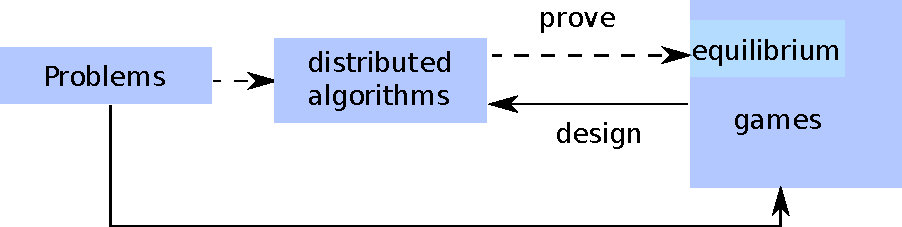
\includegraphics[width=\linewidth]{game_distributedalgorithms.pdf}
  \caption{The two ways that game theory is involved in problem solving}
\label{game_distributedalgorithms}
\end{figure}

Along the dashed line and arrow, proposed distributed schemes can be examined under the game theoretic framework.
In this way, a distributed algorithm is analysed by looking into the interaction among the users which operate the algorithm, and check whether the system reaches a desirable equilibrium, \ie the individuals not only improve their own performance but also improve the global welfare of the complete system.
In most cases, we can also inverse the this procedure to obtain distributed algorithms in CRN from certain known games~\cite{altman_Smodel_pc_2003}.
As the solid line with arrow points shows, given a known game which holds preferred properties such like fast convergence to equilibrium, or the game only has a single equilibrium which is also the global optimal, we can formulate our problem in CRN into that kind of game, then modify the best response of the players as the distributed algorithm for the communication entities in our problem. 

In this dissertation, we look into congestion game and its applications in CRN.
We leave the introduction of game theory and game models in the Chapter~\ref{background}.



\section{Problem Statement and Research Scope}

As to the various challenging problems in CRN networks, adopting centralized or decentralized solutions is largely dependant on the natures of the networks, and the concrete problems to be addressed.
%Working with the TV white space is regarded as one application of cognitive radio network, which is most likely to succeed in near future.
CRAHNs consist of mobile autonomous secondary users and don't have infrastructure, besides, the network topology evolves with time due to users' mobility, and the ungovernable primary users' activity leads to temporal spectrum availability. 
Because of these factors, secondary users execute concurrently based on the local information, then the distributed scheme becomes the natural choice to manage the CRAHN to convey services.
%
%In the networks with structure, \eg the commercial cellular networks work with licensed spectrum, the network they operate in centralized manner to provide services meeting QoS criterion.
%As to the cellular networks working with unlicensed spectrum opportunistically, there exists a centralized data base to regulate the working channel for secondary users~\cite{crn_futurecellular_2014}.
The opening of TV white space attracts people and organizations to build cellular networks to launch various services.
A data base is required to register the fixed and mode II TVBDs~\cite{crn_futurecellular_2014}, but it is not supposed to afford the computation on the resources for each TVBD.
Besides, the operation of TVBDs is carried out by different users or operators, thus it is not feasible for the centralized entity to coordinate the devices and assign the network sources to them.
Hence distributed scheme is also necessary in the utilization of TV white spectrum.
%There is one centralized database which is required by regulations and standards, thus it is possible to conduct certain centralized solutions on it.
%But the owners of the cellular networks have different or conflicting interests, \eg the networks compete for resources, besides, there maybe secondary users which start or cease to use the TV white spectrum,  
%Last but not least, the TVBDs may join or leave the network, \ie start to transmit or cease transmitting, which brings dynamics to the network, thus centralized scheme
%Actually, the majority of the research in cognitive radio domain is carried out with distributed manner.
%In CRAHNs, there are no centralized utility, and the spectrum sensing is necessary for every secondary user.

As introduce in Sections~\ref{gametheory_crn} and \ref{distributed_scheme}, game theory is suitable to design distributed schemes.
Suitable game models can be used to analyse distributed scheme in terms of the final state of the system after convergence, and the speed to reach the equilibrium.
In this thesis, we propose distributed schemes to solve the pressing problems about utilizing the unlicensed spectrum.
Except for the provisioning of services, we are also interested in the mechanism the distributed algorithms.
In particular, we look into the following questions, 
Does the distributed algorithm converge? 
If the algorithm converges, in which state the algorithm finally ceases, and how robust and quick the convergence process is?
To answer these questions, we turn to game theory, in particular, the recent progress of congestion game models for help.




\subsection{Research Questions}
Based on the description of the challenges in cognitive radio networks, we formulate two research questions which will be answered in this thesis.

Question 1 - When distributed algorithms are necessary due to the specific properties of a problem, how to guarantee the convergence and performance? How to design utility function to make use of the game model when designing the algorithm?

Question 2 - What are the strengths and weaknesses of the distributed algorithm compared with other schemes, in particular, the centralized scheme?

%Question 1 - How to design distributed solution with assistance of game model, so that to make full use of the TV spectrum with the regulated network structure? 
%
%Question 2 - How to design distributed solution with assistance of game model, to form robust clusters against primary users' unpredictable activity, so that maintain the benefits brought by cluster structure?
%
%Question 3 - How to make use of the statistic information of the spectrum availability, so as to realize light weight geographic routing in CRN?



\subsubsection{Contributions}
In this thesis, we answer the aforementioned research questions by making the one to one contributions.

Contribution C1 - We apply congestion game in the new domains to solve the concrete problems in CRN, and design distributed schemes with which the secondary users comply with the behaviours of players of the congestion game.
With the properties of congestion game, we investigate the concerns on convergence and overhead of the proposed distributed algorithms.

Contribution C2 - We compare the performance of the proposed scheme with other distributed schemes and centralized scheme.



%We briefly introduce the contribution of this dissertation by addressing the aforementioned questions.
We demonstrate how to refrain the overhead and fasten the convergence process, especially, we utilize the available game models to design distributed algorithms which have the desired these properties.
These contributions are illustrated in the process of solving three concrete technical problems.
%We investigate the differences between decentralized and centralized schemes in terms of several criteria, \ie performance, overhead, computation time, etc..
Figure~\ref{overview} illustrate the relation between contributions and the concrete technical problems to be addressed in this thesis.
\begin{figure}[h!]
  \centering
  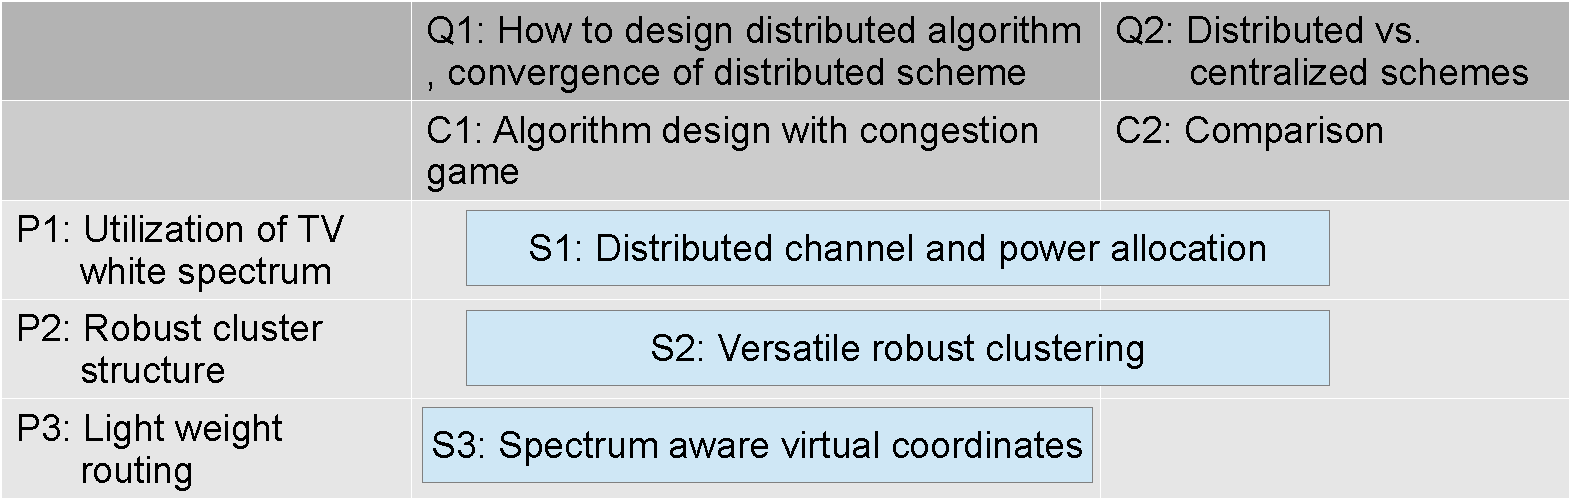
\includegraphics[width=\linewidth]{overview.pdf}
  \caption{Overview of the problems and contributions, and the concrete problems addressed in this thesis.}
\label{overview}
\end{figure}
%We focus on the distributed solutions for several correlated fundamental problems in CRN.
%The interaction among autonomous secondary users is a common scene in CRN as there usually lacks central controller.



%On physical layer, the secondary users endeavour to maximize their performance by choosing the channel and power, and meanwhile the accumulative interference caused on primary users should be below a threshold.
%How to refrain the accumulative interference from exceeding the threshold of primary users is a critical question, and how does the distributed decision on channel and transmission power improves performance is worth considering.
%After forming the connected network with the chosen channel and transmission power, obtaining the cluster structure brings many benefits, \ie more accurate spectrum sensing results due to local cooperation and facilities on other service provisioning.
%How to form such clusters which can survive in front of the unpredictable activity of primary users is challenging.
%Having had solid CRN infrastructure, it is time to deliver services via routing.
%A light weight routing tailored for CRN is needed.
%In the following sections, we will introduce the problems in Figure~\ref{problemLocation} in details.
\subsection{Research Scope}
This thesis doesn't target new properties of games, or new games, instead the available knowledge of games are utilized to solve the pressing challenges existing in cognitive radio networks.
In particular, we bring the congestion game out of the routing problem~\cite{Ackermann06purenash, Papadimitriou:2001:AGI}, where the congestion game is proposed and analysed.
We apply congestion game to solve channel allocation and network structure formation problems by designing suitable utility functions for the network units.

The concrete technical challenges addressed in this thesis are shown in Figure~\ref{problemLocation}, which reside in physical layer, media access layer (\gls{mac}) layer and network layer~\cite{osi}. 
These questions are individually orthogonal, but as pressing problems in each layers, they together form a test field to check the feasibility of distributed solutions.

\begin{figure}[h!]
  \centering
  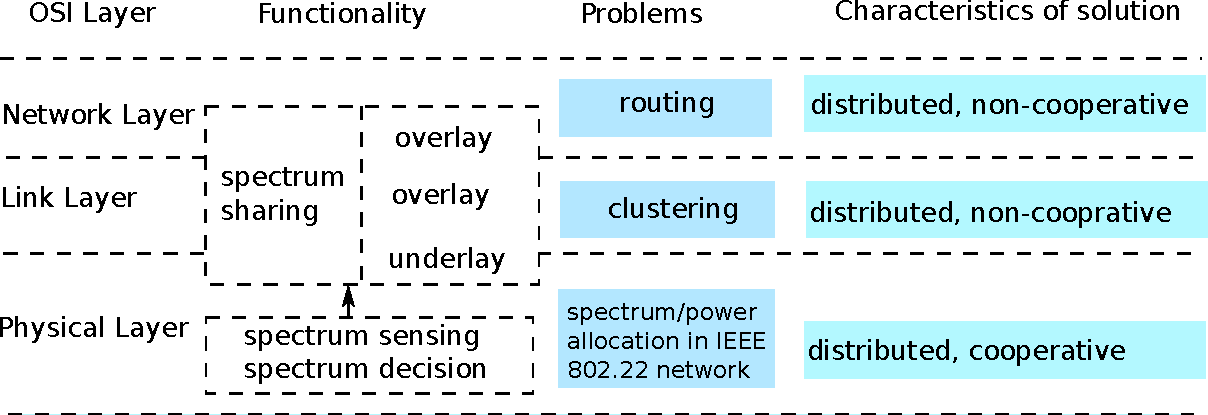
\includegraphics[width=\linewidth]{problemLocation.pdf}
  \caption{Spectrum management and the examples discussed in this thesis, congestion game is applied in two of them.}
\label{problemLocation}
\end{figure}

\subsubsection{Problem 1: Utilization of TV White Spectrum}
%\subsubsection{Utilize TV White Space}

 %Considering that secondary base stations are likely to be from different administrative domains, a distributed solution would be required. And that makes us turn to game theory and the separation of the problem into two different ones. 


%As introduced in Section~\ref{ieee80222}, the TV white spectrum has appealing characteristics for secondary users, for instance, the TV spectrum spans wide frequency range, it is not used by TV services frequently and the spectrum availability lasts relatively longer.
There are several problems in the current regulations and standards which are proposed on the utilization of TVWS.
First, most of these proposals rely on the centralized database to manage the spectrum usage in a centralized manner.
This paradigm is not suitable when the TVBD belong to different business bodies, \ie operators.
Thus, a centralized resource allocation is infeasible.
Next, the current usage of TVWS is prudent, \ie on working channel and transmission power as introduced in Section~\ref{TVWS}.
These conservative measures on the transmission power restrict the full utilization of TV spectrum.
Third, although the transmission power of TVBD is restricted, the interference between TVBDs is not given consideration by any regulation or standard.
%In fact, as the interference caused between co-channel transmitters may not be symmetric, 
In fact, the channel allocation problem we encountered in this problem is unique as the transmission power for each user and on each channel is different.
In other words, the symmetric interaction doesn't exist, thus the solutions proposed for the channel assignment problems in conventional networks, \eg ad hoc networks, or mesh networks don't work any more.
% \ie transmission power is identical for all users, and the propagation path loss is reciprocal. 
The asymmetry disables the heuristic distributed schemes provided in~\cite{Ko_DistributedCA}, and makes channel allocation problem not to fit into the congestion game model proposed in~\cite{allerton08_liu} which is the first paper to discuss channel allocation from the respective of game theory.
%Up to our knowledge, there is no work coping with co-existence between secondary base station with both primary TV broadcasters and other base stations.

%Each base station working with TVWS needs a certain transmission power and a certain spectrum.
%The decision should maximize performance of terminals in this cell under interferences from TV broadcasters and other secondary base stations, meanwhile, the TV receivers should be protected.


%In this thesis, we propose a solution for the joint power and channel allocation problem for the base stations in a WRAN network.


%This is very applicable as TV spectrum usage changes slowly, and the spectrum usage by TV stations is scheduled.
%the geographic location approach together with central database becomes more appealing in TW White Space (TVWS) utilization scenario. 
% FCC regulates portable secondary users to operate from channel 21 (512 MHz) to 51 (698 MHz), with the exception of channel 37. As to fixed secondary usage, the allowed spectrum band is from TV channel 2 (54 MHz) to TV channel 51, with TV channels 3, 4 and 37 being prohibited. Thus, the available TV spectrum is about 600 MHz wide. Compared to conventional unlicensed ISM bands in the 2.4 GHz and 5 GHz band, all together TVWS has more to offer.


\subsubsection{Problem 2: Robust Cluster Structure in Ad Hoc Cognitive Radio Network}
Clustering is an important paving stone for the practical utilization of the unused portions of the licensed spectrum.
Forming clusters with the secondary users which have proximity of geography and other properties produces several benefits.
First, it is more efficient to solve common control channel (\gls{CCC}) problem with cluster structure.
Dedicated and static CCC which is allocated to all users is regarded to be under utilization and contrary to the opportunistic access paradigm.
Whereas, cluster based approaches group CR users into clusters based on their similarity of available unlicensed channels, so that different common channels are used in various clusters to convey control messages~\cite{Lazos09}.
%whereas communication rendezvous, \ie the process to establish control channel between two CR users before they can communicate is proposed to be a economic solution.
%Within one cluster which is composed with CR nodes with similar available unlicensed channels, communication rendezvous can be accomplished within in shorter time~\cite{CommunicationRendezvous_ToN13}.
Second, cluster structure facilitates cooperative sensing and increases the sensing reliability~\cite{Sun07_clustering_spectrum_secsing}.
Third, cluster structure supports coordinated channel switching and routing in ad-hoc cognitive radio networks~\cite{cluster_routing_2013ICC}.

The benefits promised by cluster structure is challenged by the ungovernable (from the perspective of secondary users) activity of primary users.
%The first is the abundance of common control channels within cluster should be achieved.
If the members of one cluster have to vacate all the CCCs due to primary users' appearance, the cluster can not be maintained any more.
But the cluster survives if all the cluster members can migrate to another CCC after one CCC is occupied by primary user.
Thus, a large number of CCCs within cluster means high robustness against primary users.
Unfortunately, related works~\cite{Zhao07,Affinity_clustering_09icccn,Consensus_based_clustering12,clustering_globecom11} fail to pay attention to this issue.
%Besides, more control channels makes multiple concurrent transmission within cluster possible.
%In this thesis, a distributed clustering algorithm which is especially designed to support robustness under active primary users is proposed.
There is a pressing need for one distributed clustering scheme, which should fulfil the following requirements.
First, the execution of the scheme should be finished quickly, so that the scheme can react quickly enough to the primary users' activity.
next, the scheme should achieve a proper compromise between the number of CCCs and cluster sizes.


%\item Efficient channel allocation scheme within and among clusters is needed, so that communication rendezvous between two clusters is quick. 
%Communication rendezvous means the process to establish control channel between two clusters before they can communicate .
%\cite{LIU_TMC11_2} proposes channel allocation in round robin manner, but it causes long time on communication rendezvous.
%\end{itemize}
%
%These requirements will be fulfilled by the scheme proposed in this thesis.

\subsubsection{Problem 3: Light Weight Routing in CRN}

Recent measurement in~\cite{measurement_Palaios14} shows the spectrum occupancy doesn't have significant spatial correlations between different locations.
It follows that licensed spectrum is used by primary users heavily in some areas, whereas in the other areas licensed spectrum is available over longer timespan for secondary users to use.
It is obvious to see that a routing path is better to go through the areas where primary users occupation is lower, as this alleviates or avoids the burden to cope with the fast changing or totally occupied spectrum when forwarding packets potentially with latency requirements.
Modified version of geographic routing is ale to avoid the primary user influenced area, but it is myopic.
%Geographic routing is a natural choice to realize this geography sensitive routing path, .
%Geographic routing is light weight regarding the determination of next hop, and achieves high scalability in various wireless networks~\cite{geoRouing-qos-2009}. %
%Merely knowing the geographic locations of its neighbours and the destination, a node is able to locally choose the next hop which has the smallest distance to the destination.
%As a result, control messages for route discovery are not necessary, and since the routing state maintained per node is independent on the network size, geographic routing scales perfectly.
%However, in CRN dynamic link state renders geographic routing unsuccessful since packets are forwarded to the destination along the shortest path rather than avoiding areas heavily influenced by primary users.
%Coordinates indicate not only the physical distance among SUs, but also the transmission opportunities in between could leverage the strengths of geographic routing even in CRNs.
considering the available spectrum is geographically heterogeneous, applying geographic routing alike routing schemes in CRAHN is appealing, but the supporting coordinate system is not complete.
How to make light weight geographic routing work well in CRN is the problem to be addressed.







%\subsubsection{Solution to Problem 1: Utilization of TV white spectrum and application of game model in designing algorithm}
%
%%and apply it on different cognitive radio networks.
%%rethink channel allocation problem from the perspective of game theory, particularly,
%
%In term of providing solution to fully exploit TV white space complying with IEEE 802.22 standard, we propose a complete set of methods to regulate the upper bound of transmission power, working channel and power.
%%Both FCC regulation and 802.22 standard try to make TVBD transparent to incumbent users, but as long as TV system is not affected, i.e. certain quality of service is fulfilled, the strict restriction on unlicensed users can be relaxed so that more TVWS can be provided~\cite{multipleIntf_pimrc11}. 
%%Abiding by the operation paradigm using data base, we investigate the maximal downlink transmission power for TVBDs by solving optimization problem where the cumulative interference on TV receivers is under a threshold.
%Our solution makes full use of the current network structure, strictly protect primary users with a centralized scheme which is conducted in the centralized database.
%Proposed scheme also considers the necessity of distributable execution which decides the working channel and transmission power.
%
%As to the channel allocation problem, we innovatively formulate this problem in to a canonical congestion game, and design efficient distributed channel selection strategy with the assistance of the centralized database.
%The successful practice of congestion game in this problem is enlightening for the application of congestion game in other problems where asymmetric interaction exists.
%
%%According to 802.22 regulation, spectrum allocation is done centrally in TV database, this is not realistic when TVBDs belong to different economic interest groups, thus a distributed solution is needed.
%%We propose efficient distributed scheme to allocate the TV channels in order to improve the quality of service of TVBDs.
%%The major difference between our scheme and other spectrum allocation lies in that the downlink transmission power on different channel is different.
%%We formulate this problem into a canonical congestion game, and derive the distributed algorithm from the best response behaviour of the player in the game. 
%
%
%
%
%
%
%\subsubsection{Solution to Problem 2: Versatile robust clustering in CRAHN}
%%We investigate the robust clustering problem thoroughly.
%Our proposed distributed clustering scheme achieves robust cluster structure against primary users.
%Furthermore, the clustering algorithm is versatile enough to fulfil other requirements, \ie fast convergence, less signalling and cluster size control.
%
%Congestion game model is adopted during the algorithm design, which not only contributes the algorithm design directly, but also provides guarantee on convergence and convergence speed.
%
%%We propose a decentralized clustering approach, which is able to form clusters whose sizes are not far away from the desired size, and the generated clusters are more robust than other robust clustering scheme, \ie more secondary users residing in clusters against increasing affection from primary users.
%%Compared to previous work, our proposed scheme involves much less control messages, and the generated clusters are significantly more robust.
%%We formulate one procedure of the scheme into a singleton congestion game, which permits Nash equilibrium when CR users adopt  best response strategy. 
%%building more homogeneous clusters with respect to their size and forcing nodes with a high connectivity degree to the border of a cluster (making the cluster therefore more robust regarding connectivity loss to its neighbor).
%%For our scheme we can prove convergence in cluster formation phase and resolve ambiguities with respect to cluster membership in a game-theoretic setting. 
%%On the basis of proposed scheme, we propose a light weighted version of ROSS, which requires exchanging less overheads.
%%We leave the channel selection undiscussed.
%
%
%
%
%
%
%
%\subsubsection{Solution to Problem 3: Spectrum aware virtual coordinates and geographic routing in CRN}
%
%%In this paper we propose SAViC, spectrum aware virtual coordinates for secondary users in multi-channel multi-hop CRN where secondary users are source limited.
%We design spectrum virtual coordinate for CRN, which is not only independent on geographic position, but decided by connection quality among nodes, for instance, channel availability, link quality or hop numbers.
%With this new coordinate, Euclidean distance between two secondary users reflects the availability of unlicensed channel between them.
%Then the geographic routing can run with this coordinate system as the spectrum virtual coordinate contributes a large part to the decision on next hop.
%%The proposed virtual coordinate depicts the availability of licensed spectrum influenced by primary users, on top of which geographic routing decides the next hop with Euclidean distance metric, and unconsciously detours the primary affecting area, or cuts through the area with better access opportunity.
%%This routing paradigm imposes little computation and communication cost on secondary users after assigning virtual coordinate, besides, it doesn't need real geographic location which is employed in ~\cite{search_geo_routing_chowdhury, routing-crn-jsac12}.
%%
%%This scheme is composed with two steps,
%%\begin{itemize}
%%\item Design virtual coordinates so that virtual coordinates of any two secondary users reflect both geographic distance and opportunistic spectrum availability between them.
%%We design them based on statistics of primary user’s ON/OFF states which are obtained from local spectrum sensing.
%%
%%\item After deciding on the next hop, we adopt a lightweight heuristic method to decide which channel to transmit packet when multiple licensed channels exist in the network.
%%
%%
%%\end{itemize}

%%To summarize, as the Euclidean distance between two secondary users based on spectrum aware virtual coordinate reflects the availability of unlicensed channel in between from the angel of historical statistics, virtual coordinate contributes a large part to deciding on the on the next hop. 



\section{Outline}
The structure of this thesis is as follows.
In chapter 2, we introduce the theoretical tools used in design algorithms, \ie game theory and optimization. 
Chapter 3 introduces the work on utilization of TV white space.
The robust clustering scheme is introduced in Chapter 4.
In Chapter 5, virtual coordinate based on geographic routing is designed and geographic routing runs on the top of it.
Finally, Chapter 7 concludes the thesis by summarizing our contributions and discussing the future work.




